\documentclass{article}

\usepackage[normalem]{ulem}
\usepackage{fancyhdr}
\usepackage[parfill]{parskip}
\usepackage{tikz}
\usepackage{multicol}
\usepackage{SIunits}
\pagestyle{fancyplain}
\usetikzlibrary{shapes, patterns}

\title{3.5.3 Muscles}
\author{Todd Davies}
\date{\today}

\begin{document}

\rhead{3.5.3 Muscles}
\lhead{\today}

\maketitle

\section*{The structure of muscle}
\thispagestyle{empty}

Muscles are made up of many increasingly small subdivisions as shown below:

\begin{center}
	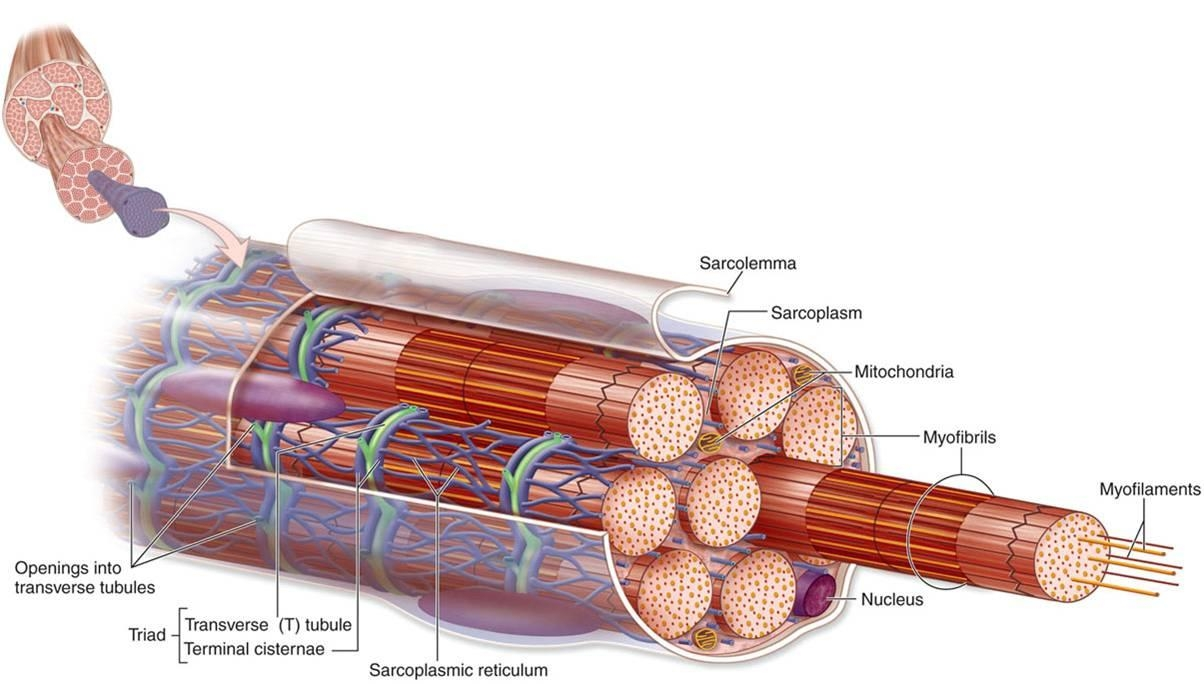
\includegraphics[scale=0.35]{sceletal_muscle}
\end{center}

In the top left corner, you can see the whole muscle, then a bundle of muscle
fibres, then a single muscle fibre. The single muscle fibre is shown in greater
detail.

Each muscle fibre has many smaller myofibrils, and myofilaments are contained
within these. There is no distinct seperation between muscle cells. They all
merge into one, and in doing so share their nuclei. They also have a shared
cytoplasm, which is called a {\bf sarcoplasm}.

\subsection*{The microscopic structure of muscle}

Each myofibril contains two types of protein filament (myofilaments), {\bf
actin} and {\bf myosin}.

Actin is thin and consists of two strands twisted around each other, while
myosin is thicker and has many bulbous heads projecting to the side.

The outside of a muscle fibre has visible striations. The alternating bands of
dark and light colour are called anisotropic (A-bands) and isotropic (I-bands)
respectively.\marginpar{L{\bf i}ght={\bf i}sotropic\\D{\bf a}rk={\bf
a}nisotropic}

The anisotropic bands appear dark since the actin and myosin filaments overlap
in these regions.

\begin{center}
	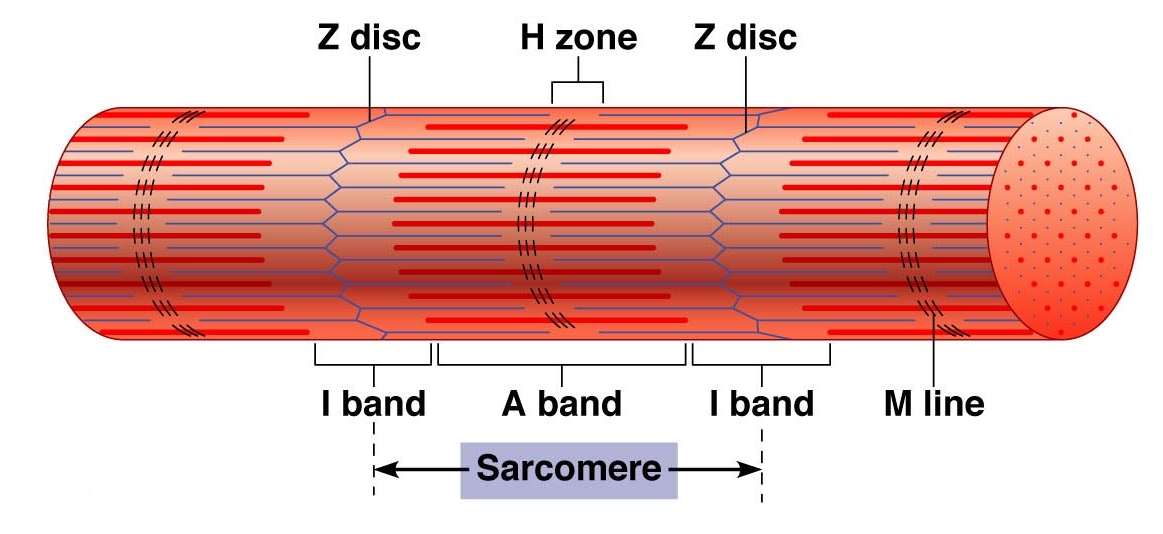
\includegraphics[scale=0.65]{muscle_structure}
\end{center}

\subsection*{Types of muscle fibre}

There are two types of muscle fibre. The ratio of the different types of fibre
in a muscle depends on what muscle it is, and the genotype of the organism.

\subsubsection*{Slow twitch fibres}

Slow twitch fibres contract slowly and provide less powerful contractions over a
long period of time. They are of high density in muscles such as the calf that
are involved in keeping upright. They are suited to aerobic resperation and have
a very good blood supply in order to avoid buildups of lactic acid.

They also have a large store of myoglobin, a rich supply of glycogen and lots of
mitochondria to deliver ATP.

\subsubsection*{Fast twitch fibers}

Fast twitch fibers are able to contract rapidly and produce powerful
contractions, but for only a short period of time. They are common in muscles
that usually do short bursts of intense activity (such as lifting), for example,
the bicep.

They have lots of thick myosin filaments, a high concentration of enzymes
involved in anaerobic resperation, and lots of
phosphocreatine.\marginpar{\raggedright Phosphocreatine is a molecule that can
rapidly generate ATP from ADP in anaerobic conditions.}

\section*{Neuromuscular junctions}

A neuromuscular junction is the point where a motor neurone meets a skeletal
muscle fibre. There are lots of these junctions along the muscle tissue, so that
all of the muscle can contract at the same time, and a strong contraction can
occur.

Not all of the motor neurones leading to a muscle need to be stimulated at the
same time. A weak contraction can be produced when only a few of the motor
neurones have impulses traveling through them.

\section*{Muscle contraction}

When a muscle contracts, the following changes occur to a sarcomere:

\begin{itemize}

	\item The I-band becomes narrower.

	\item The Z-lines move closer together. \marginpar{\raggedright Since the
	Z-lines define the limits  of the sarcomere, the sarcomere could be said to
	get shorter}

	\item The H-zone becomes narrower.

\end{itemize}

The width of the A-band stays the same, which means that the myosin filaments
mustn't get shorter (since the width of the A-band depends on the length of the
myosin filaments).

In muscle contraction, the actin and myosin filaments slide past each other,
causing the muscle to become shorter.

\begin{center}
	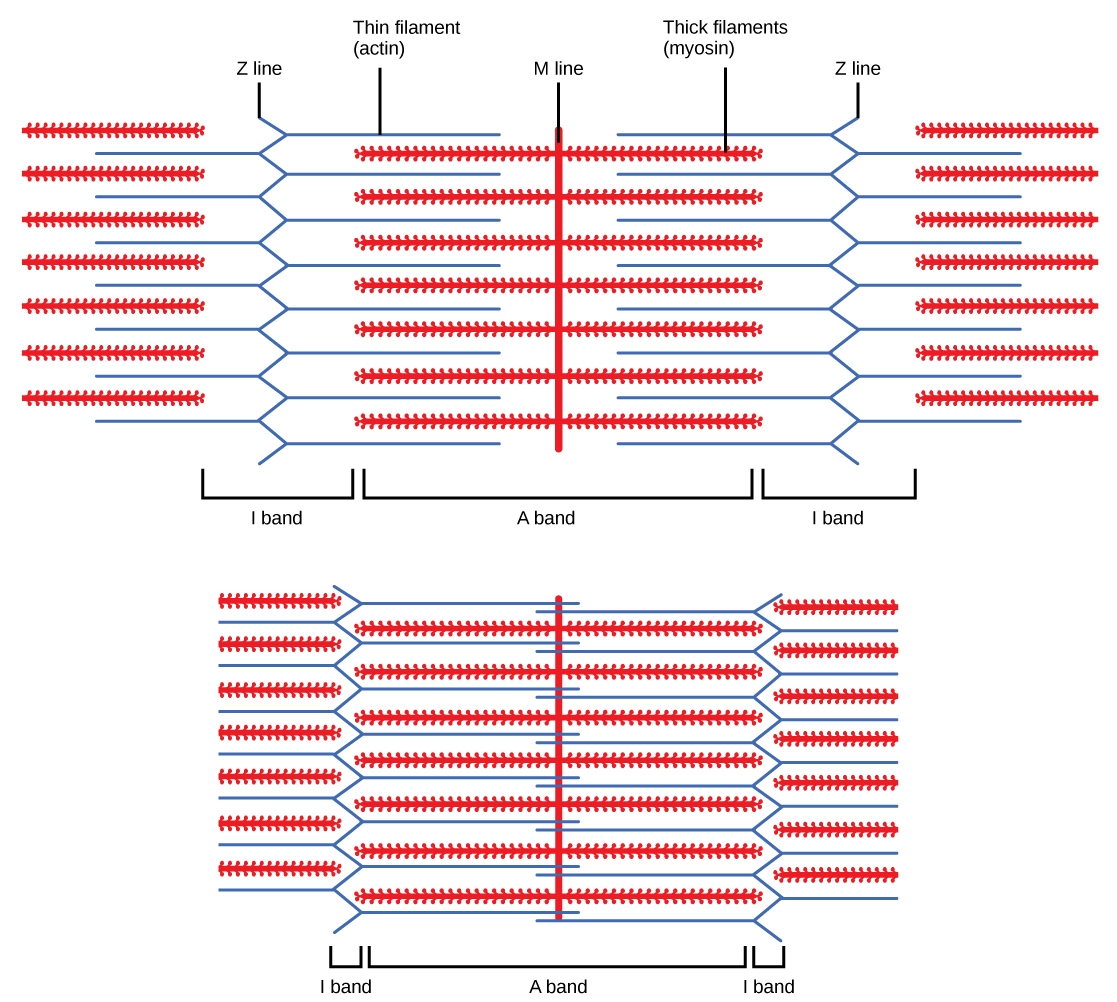
\includegraphics[scale=0.65]{contraction}
\end{center}

\subsection*{The mechanics of muscle contraction}

The structure of the three proteins that facilitate muscle contraction is as
follows:

\begin{itemize}

	\item {\bf Myosin} is up of a long tail with a two bulbous heads at one end.

	\item {\bf Actin} is a globular protein, with it's molecules arranged into
	long chains that are twisted into a helixical strand (a bit like DNA).

	\item {\bf Tropomyosin} forms thin long threads that are wound around the
	actin filaments.

\end{itemize}

In muscle contraction, the bulbous heads of the myosin filaments form cross
bridges with the actin filaments by attaching to binding sites on the actin. All
of the heads on the myosin move in unison and pull the actin filaments along the
myosin filaments. The myosin heads then detach and reset to their original
position using energy from ATP. This can happen up to 100 times per second.

\subsubsection*{Muscle stimulation}

When an action potential reaches a neuromuscular junction, calcuim ion channels
open and calcium ions flow into the synaptic knob. The calcium ions cause the
symaptic vesicles to fuse with the presynaptic membrane and release acetylcoline
into the synaptic cleft. The acetylcoline then diffuses across the synaptic
cleft into neuroreceptors embedded in the postsynaptic membrane, which causes
depolarisation.

\subsubsection*{Muscle contraction}

\begin{enumerate}

	\item The action potential travels down the T-tubules that branch out
	throughout the sarcoplasm of the muscle cell.

	\item The calcium ion channels on the endoplasmic reticulum inside the
	muscle cells (that are attached to the T-tubules) are opened by the action
	potential and calcium ions flood into the sarcoplasm.

	\item This causes the tropomyosin molecules to change their position on the
	actin strands to that the myosin binding sites are uncovered.

	\item The myosin heads now bind with the actin filament forming a cross
	bridge.

    \item The myosin heads now change their angle so that the actin filament is
    pulled along. This releases a molecule of ADP \marginpar{\raggedright N.b.
    ADP wasn't created here, it was already there to begin with.} that was
    stored on the myosin head.

    \item An ATP molecule attaches to the myosin head which detaches it from the
    actin.

    \item ATPase hydrolyses ADP from ATP which releases energy so that the
    myosin heads can return to their original position.

    \item The ADP molecule then attaches to the myosin head again ready for
    another 'stoke'.

\end{enumerate}

\subsubsection*{Muscle relaxation}

When the nervous stimulation has stopped, the calcium ions are actively
transported back into the endoplasmic reticulum using energy from the hydrolysis
of ATP. This allows tropomyosin to cover the actin binding sites again, meaning
the myosin heads are unable to bind to the actin  filaments which causes muscle
relaxation.

\section*{Energy supply during muscle contraction}

Lots of energy is used for muscle contraction in order to move the myosin heads
and to actively transport calcium into the endoplasmic reticulum. This means
that muscles have a great demand for ATP.

Most of the ATP that is used in the muscles is generated from ADP and organic
phosphate by mitochondria (aerobic resperation). However this requires oxygen,
and when a muscle is working hard, local oxygen supplies are depleted fast.

Phosphocreatine is a molecule that aids anaerobic resperation in muscles.
Phosphocreatine acts as a reserve supply of phosphate, which is able to bind to
ADP in order to reform ATP. The phosphocreatine stores are replenished when
oxygen becomes availible again, and the muscle has relaxed.

\end{document}